\documentclass{amsart}

\usepackage{amsmath}
\usepackage{cite}
\usepackage{graphicx}
\usepackage{url}

\newtheorem{theorem}{Theorem}[section]
\newtheorem{lemma}[theorem]{Lemma}
\newtheorem{corollary}[theorem]{Corollary}
\newtheorem{proposition}[theorem]{Proposition}
\newtheorem{example}[theorem]{Example}
\newtheorem{definition}[theorem]{Definition}

\newcommand{\RR}{\mathbb R}
\newcommand{\fS}{\mathfrak S}

\newcommand{\aut}{\mathsf A}
\newcommand{\pairing}{\mu}
\newcommand{\tangle}{\mathsf{G}}
\newcommand{\ptree}{\mathsf{P}}
\newcommand{\ptequiv}{\bar{\ptree}}  % Phylogenetic tree equivalence classes under the symmetric group.
\newcommand{\stpair}{\mathsf{Q}}  % Shape-tree pair.
\newcommand{\bigproj}{\tilde \pi}

% arxivness
\newcommand{\arxiv}[1]{#1}
\newcommand{\notarxiv}[1]{}

\newcommand{\FIGspr}{\
\label{FIGspr}
\begin{figure}
  \arxiv{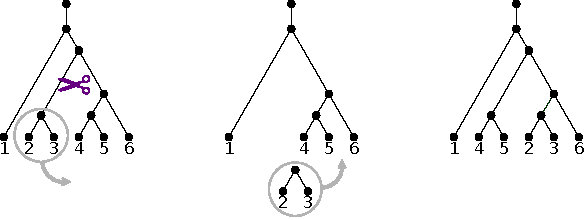
\includegraphics[width=4in]{figures/spr-definition}}
\caption{\
  A subtree-prune-regraft move.
}
\end{figure}
}


\begin{document}
\title{Symmetries of tanglegrams}
\author[Matsen]{Frederick A. Matsen IV}
\address{Fred Hutchinson Cancer Research Center \\ Seattle, WA}
\thanks{Research supported in part by National Science Foundation award 1223057 and National Institutes of Health grant R01 GM113246-01}


\date{\today}

\begin{abstract}
Many interesting discrete mathematics problems concerning phylogenetic trees are defined in terms of the relative labeling of pairs of leaf-labeled trees.
These relative labelings are naturally formalized as so-called ``tanglegrams.''
Although there has been considerable work on planar embeddings of tanglegrams, many questions remain concerning their symmetries.
Understanding symmetries of tanglegrams would give information on how many problems on relatively labeled pairs of trees there are, open up the possibility for amortized algorithms, and reveal natural symmetries of spaces associated with such problems.
In this paper we develop methods to enumerate tanglegrams up to isomorphism, and we investigate the representation of the symmetric group induced by its action on tanglegrams.
\end{abstract}

\maketitle


\section{Introduction}
As a motivating example, we consider the problem of computing the \emph{subtree-prune-regraft} (SPR) distance between two leaf-labeled phylogenetic trees.
An SPR move cuts one edge of the tree and then reattaches the resulting rooted subtree at another edge (Figure~\ref{FIGspr}).
The SPR distance between two (phylogenetic, implying meaning leaf-labeled) trees $t_1$ and $t_2$ is the minimum number of SPR moves required to transform $t_1$ into $t_2$.

Clearly the distance between two such trees does not depend on the actual labels of $t_1$ and $t_2$.
For example, one could exchange numbers labeling the two trees with their corresponding taxonomic names.
Or one could simply permute the numerical labels of the leaf nodes, which would result in the same problem if the permutation was applied identically on both the starting and ending trees.
Furthermore, a path made by SPR moves made by intermediate trees between the two trees could also have its labels permuted in order to give a path between the trees with permuted leaf labels.
Thus, all of these problems do not concern the actual leaf labels as such, but rather use the leaf labels as markers that can be used to map leaves of one phylogenetic tree on to another: the problem and its solutions are actually defined in terms of a \emph{relative} leaf labeling.
\FIGspr

Such discrete mathematics problems and objects defined in terms of pairs of labeled combinatorial objects are ubiquitous in computational biology.
In addition to SPR distances and their cousin distances formed by \emph{nearest-neighbor-interchange} and \emph{tree bisection and reattachment} \cite{wiki:treeRearrangement}, we have their corresponding biological questions concerning ``supertree'' reconstruction \cite{Whidden2014-ku} and reconciliation of gene transfer networks \cite{Boon2013-mc}.
Because such moves are used in both maximum-likelihood heuristic search and Bayesian Markov chain Monte Carlo (MCMC) tree reconstruction, the geometry of phylogenetic trees under such moves has substantial consequences in terms of phylogenetic tree reconstruction \cite{Whidden2014-yt}.

Another line of inquiry in computational biology concerns species delimitation, which can naturally be phrased in terms of inference of a partition of labeled objects.
In an analogous way, scientists use MCMC to explore the posterior on such partitions \cite{Yang2010-kc}, and comparison of the results can be performed using distances between the partitions via distances such as \cite{Gusfield2002-il}.
These partitions can also be thought of as a certain type of leaf-labeled tree of height two, and thus they also form a problem concerning relative leaf labeling of phylogenetic trees.

The concept of a pair of phylogenetic trees with a relative leaf labeling is essentially the same as the graph-theoretic notion of a \emph{tanglegram}.
A tanglegram is a pair of trees on the same set of leaves with matching leaves in the two trees joined by an edge. \cite{Venkatachalam2010-zh}.
There has been extensive work concerning tanglegrams, focusing on the problem of drawing them in a way that has minimum crossings \cite{Buchin2008-lc,Lozano2008-tp,Bansal2009-ni,Bocker2009-xl,Fernau2010-an,Venkatachalam2010-zh}.

In this paper we explore the mapping of pairs of leaf-labeled trees into the set of tanglegrams and explore the action of the symmetric group on tanglegrams.
We are able to write down isomorphism classes in terms of the symmetries of the two phylogenetic trees they contain.
Furthermore, tanglegrams are equipped with a natural action of the symmetric group on the leaf set, which we describe.
We use the SAGE mathematics software \cite{SteinJoyner2005} to further explore these symmetries, resulting in tables of representatives of tanglegrams and their multiplicities, as well as the irreducible representations of the symmetric group defined by the action on tanglegrams.


\section{Formalism}
All of our trees will be bifurcating (i.e.\ internal nodes have degree three), and without leaf labels if not otherwise specified.
I don't think the bifurcating matters, although it will be nice

Note that we can't completely treat a rooted tanglegram as unrooted for the purposes of automorphism: we don't want to move a root edge onto a leaf edge.

start with labeled definition?
Labeled trees and elements of $\fS_n$
Although these labels don't have any real significance, they are convenient to use when referring to leaves.

\begin{definition}
\label{def:tanglegram}
An $n$-\emph{tanglegram} is an ordered triple $(t_1, t_2, \pairing)$ where $t_1$ and $t_2$ are trees with $n$ leaves, and $\pairing$ is a bijection from the leaves of $t_1$ to those of $t_2$ which we will call the ``pairing.''
Let $\tangle_n$ denote the set of $n$-tanglegrams.
\end{definition}
Note that we have not specified whether the trees in the definition are rooted or not.
There is no essential difference between these two cases because if present, as the root of $t_1$ is naturally paired with the root of $t_2$.
Thus we will assume that the trees are rooted.
Note that our definition considers $(t_1, t_2, \pairing)$ and $(t_2, t_1, \pairing^{-1})$ as different maps.
We can also consider an unordered tanglegram, or \emph{utanglegram}, by identifying them.

A common way of specifying a tanglegram is by specifying two trees with the same leaf labels, with the idea that pairs of leaves that share a label are paired in the tanglegram.
These labels do not themselves carry information for the tanglegram but just to make these connections, motivating the definition above in terms of a bijection.
However, for our purposes it will be useful to sometimes refer to a tanglegram as if it consists of a pair of trees on the same leaf labels such that pairs of leaves that share a label are paired in the tanglegram.

We can also construct a (unlabeled) graph $g(x)$ for a given tanglegram $x$ by connecting corresponding leaves.


\section{Symmetric group action and tanglegram symmetries}
Let $\fS_n$ denote the symmetric group on $n$ items.
We define the action of $\fS_n$ on $n$-tanglegrams to be such that an element of the symmetric group reorders the image of the leaf-to-leaf mapping.
That is, for $\sigma_n \in \fS_n$ and $(t_1, t_2, \pairing) \in \tangle_n$,
\[
\sigma \cdot (t_1, t_2, \pairing) := (t_1, t_2, \sigma \cdot \pairing),
\]
where $\sigma \cdot \pairing$ is the leaf-to-leaf mapping obtained by rearranging the image of $\pairing$ according to $\sigma$, i.e.\ $(\sigma \cdot \pairing)(x) = \sigma(\pairing(x))$.

Thus far we have groups acting on the left, such that $(\sigma \tau) \cdot x = \sigma \cdot (\tau \cdot x)$.
When applied to a pairing $\mu$ this means that the group action happens on the image of $\mu$, i.e.\ the leaves of $t_2$.
However, we can effectively act on the leaves of $t_1$ by conjugating with $\pairing$:
\begin{equation}
\label{eq:rightAction}
(\pairing \alpha_1 \pairing^{-1}) \cdot x
= (t_1, t_2, \pairing \alpha_1 \pairing^{-1} \pairing)
= (t_1, t_2, \pairing \alpha_1)
\end{equation}

Given a (rooted) phylogenetic tree $t$ let $\aut(t)$ be its leaf automorphism group.
That is, if $t$ has $n$ leaves (excluding the root if it exists) these are the elements $\alpha$ of $\fS_n$ that do not change $t$ when applied permute its leaves.
Because every tree has at least one cherry (a subtree of size 2), the automorphism group of every tree has at least the symmetry of exchanging the two leaves of that cherry.

These symmetries determine the symmetries of the tanglegram.
It is clear that for $\alpha_2 \in \aut(t_2)$, and $x = (t_1, t_2, \pairing)$,
\[
\alpha_2 \cdot x = (t_1, t_2, \alpha_2 \pairing) = x.
\]
Furthermore, as with \eqref{eq:rightAction}, given $\alpha_1 \in \aut(t_1)$,
\[
(\pairing \alpha_1 \pairing^{-1}) \cdot x = (t_1, t_2, \pairing \alpha_1) = x.
\]
Define the group $\aut(x)$ of an $n$-tangle $x = (t_1, t_2, \pairing)$ to be the subgroup of $\fS_n$ generated by $\pairing \aut(t_1) \pairing^{-1}$ and $\aut(t_2)$:
\[
\aut(x) = \langle \pairing \alpha_1 \pairing^{-1}, \alpha_2 \mid \alpha_1 \in \aut(t_1), \alpha_2 \in \aut(t_2) \rangle.
\]

It is clear that each element of $\aut(x)$ induces an automorphism of the graph $g(x)$ by leaving the trees fixed, and permuting the connections between them as per the group action on tangles.
Now let $\tilde \sigma$ be an automorphism of $g(x)$ which maps the leaf set of each tree to itself.
Because the leaves map to themselves, the internal nodes of the trees map to themselves.
(If they didn't then there would have to be exchange of nodes between trees, and thus they would have to "hop over" the leaves.)
Thus any such graph automorphism must be a pair automorphisms $\alpha_1, \alpha_2$ of the trees.
There is a one-to-one correspondence between the elements of the symmetric group and their matching graphs.
Thus if it is an isomorphism of $\aut(x)$ then it induces an identical $\mu$.
This shows:
\begin{proposition}
For any tanglegram $x$ that does not have degree two edges, $\aut(x)$ is the exactly group of graph automorphisms of the graph $g(x)$ that fix the leaf sets of $x$.
\end{proposition}



\section{Computation}
How to describe the ensemble of tanglegrams.
For the purposes of classification it is more straightforward to specify tanglegrams in terms of standardized trees and a permutation rather than in terms of the bijection in Definition~\ref{def:tanglegram}.
Assume we are working with $n$ taxa.
Let $\ptree$ be the set of \emph{phylogenetic} trees on $n$ leaves.
Let $\ptequiv$ be the equivalence classes of $n$ taxon phylogenetic trees under the action of the symmetric group $\fS_n$ on the leaf labels, and let $k$ be the number of such equivalence classes.
These are in one-to-one correspondence with the (graph-isomorphically-) distinct unlabeled bifurcating trees.

Let us fix representatives $\{s_i\}_{i=1,\ldots,k}$ of the equivalence classes $\ptequiv$.
Any tree $t$ has a representative $s_i$ of its equivalence class in $\ptequiv$, and there is a corresponding $\sigma \in \fS_n$ that maps the leaf labels of $s_i$ to those of $t$.
We will call this $\sigma$ the \emph{standard permutation} of $t$.

Consider two phylogenetic trees $t_1, t_2$ with representatives $s_{(1)}$ and $s_{(2)}$ and standard permutations $\sigma_1$ and $\sigma_2$.
The group element $\sigma_2^{-1} \, \sigma_1$ maps the leaves of $s_{(1)}$ to the leaves of $s_{(2)}$ that they correspond to in the $(t_1, t_2)$ tanglegram.
Indeed, $\sigma_1$ maps the leaves of $s_{(1)}$ to the corresponding leaves of $t_1$, $t_1$ and $t_2$ have identical leaf labels for leaves connected in the tanglegram, and $\sigma_2^{-1}$ maps the leaves of $t_2$ to the corresponding leaves of $s_{(2)}$.
Thus the triple $(s_{(1)}, s_{(2)}, \sigma_2^{-1} \, \sigma_1)$ defines the tanglegram formed by the two phylogenetic trees $t_1$ and $t_2$.
In terms of the standardization this is
\[
\sigma \cdot (s_{(1)}, s_{(2)}, \sigma_2^{-1} \, \sigma_1) \mapsto (s_{(1)}, s_{(2)}, \sigma_2^{-1} \, \sigma \sigma_1).
\]



However, there are additional symmetries defined by automorphisms of the two trees: any pair of automorphisms $\alpha_1 \in \aut_1, \alpha_2 \in \aut_2$ induce an isomorphic tanglegram $(s_{(1)}, s_{(2)}, \left(\sigma_2 \alpha_2 \right)^{-1} \, \sigma_1 \alpha_1)$.
Define the \emph{standardization} of a (labeled) tanglegram to be the triple
\begin{equation}
\label{eq:orbit}
\left(s_{(1)}, s_{(2)}, \left\{(\sigma_2 \alpha_2)^{-1} \, \sigma_1 \alpha_1 : \alpha_1 \in \aut_1, \alpha_2 \in \aut_2  \right\}\right)
\end{equation}
or more simply $(s_{(1)}, s_{(2)}, [\sigma_2^{-1} \, \sigma_1])$ where the brackets imply equivalence class under the automorphisms.
The third element in this triple will be called the \emph{orbit} of the tanglegram.

There is a one-to-one correspondence between tanglegrams and standardizations.
.
Indeed, assume that we have two isomorphic tanglegrams, which we consider as a pair of labeled tanglegrams with an arbitrary label set.
The isomorphism between the two labeled tanglegrams can be expressed as a permutation $\tau$ of the leaf labels.
Each of the first trees must have the same standardization, and also the same orbit because $[\left(\tau \sigma_2\right)^{-1} \, \tau \sigma_1] = [\sigma_2^{-1} \, \sigma_1]$.
Now if we are given a standardization, we can pick a representative from the orbit and assemble the corresponding tanglegram, which is well defined because tree automorphisms do not change the underlying tanglegram.

Now given a list of trees $t_1, \ldots, t_\ell$ one can enumerate all tanglegrams formed by pairs of $t_i$ with two straightforward steps.
First, for each tree $t_i$ find a representative $s_{(i)}$ and standard permutation $\sigma_i$.
Second, create every triple $(s_{(i)}, s_{(j)}, \sigma_j^{-1} \sigma_i)$.
Third, compute the orbit \eqref{eq:orbit}.

Q: can we say anything about the number of tanglegrams?


Q: What representation is this?



\section{Acknowledgements}
This manuscript was substantially shaped by discussions with Michael Landis, Arnold Kas, and Chris Whidden.

\bibliographystyle{unsrt}
\bibliography{tangle}


\notarxiv{
\section{Figure legends}
\FIGspr
}
\end{document}

